\documentclass[a4paper,11pt,twoside]{report}
\usepackage[left=3cm,right=2cm,top=2.5cm,bottom=2.5cm]{geometry}
\usepackage{graphicx}
\usepackage{verbatim}
\usepackage{latexsym}
\usepackage{mathchars}
\usepackage{setspace}

\setlength{\parskip}{\medskipamount}  % a little space before a \par
\setlength{\parindent}{0pt}	      % don't indent first lines of paragraphs
%UHEAD.STY  If this is included after \documentstyle{report}, it adds
% an underlined heading style to the LaTeX report style.
% \pagestyle{uheadings} will put underlined headings at the top
% of each page. The right page headings are the Chapter titles and
% the left page titles are supplied by \def\lefthead{text}.

% Ted Shapin, Dec. 17, 1986

\makeatletter
\def\chapapp2{Chapter}

\def\appendix{\par
 \setcounter{chapter}{0}
 \setcounter{section}{0}
 \def\chapapp2{Appendix}
 \def\@chapapp{Appendix}
 \def\thechapter{\Alph{chapter}}}

\def\ps@uheadings{\let\@mkboth\markboth
% modifications
\def\@oddhead{\protect\underline{\protect\makebox[\textwidth][l]
		{\sl\rightmark\hfill\rm\thepage}}}
\def\@oddfoot{}
\def\@evenfoot{}
\def\@evenhead{\protect\underline{\protect\makebox[\textwidth][l]
		{\rm\thepage\hfill\sl\leftmark}}}
% end of modifications
\def\chaptermark##1{\markboth {\ifnum \c@secnumdepth >\m@ne
 \chapapp2\ \thechapter. \ \fi ##1}{}}%
\def\sectionmark##1{\markright {\ifnum \c@secnumdepth >\z@
   \thesection. \ \fi ##1}}}
\makeatother
%%From: marcel@cs.caltech.edu (Marcel van der Goot)
%%Newsgroups: comp.text.tex
%%Subject: illegal modification of boxit.sty
%%Date: 28 Feb 92 01:10:02 GMT
%%Organization: California Institute of Technology (CS dept)
%%Nntp-Posting-Host: andromeda.cs.caltech.edu
%%
%%
%%Quite some time ago I posted a file boxit.sty; maybe it made it
%%to some archives, although I don't recall submitting it. It defines
%%	\begin{boxit}
%%	...
%%	\end{boxit}
%%to draw a box around `...', where the `...' can contain other
%%environments (e.g., a verbatim environment). Unfortunately, it had
%%a problem: it did not work if you used it in paragraph mode, i.e., it
%%only worked if there was an empty line in front of \begin{boxit}.
%%Luckily, that is easily corrected.
%%
%%HOWEVER, apparently someone noticed the problem, tried to correct it,
%%and then distributed this modified version. That would be fine with me,
%%except that:
%%1. There was no note in the file about this modification, it only has my
%%   name in it.
%%2. The modification is wrong: now it only works if there is *no* empty
%%   line in front of \begin{boxit}. In my opinion this bug is worse than
%%   the original one.
%%
%%In particular, the author of this modification tried to force an empty
%%line by inserting a `\\' in the definition of \Beginboxit. If you have
%%a version of boxit.sty with a `\\', please delete it. If you have my
%%old version of boxit.sty, please also delete it. Below is an improved
%%version.
%%
%%Thanks to Joe Armstrong for drawing my attention to the bug and to the
%%illegal version.
%%
%%                                          Marcel van der Goot
%% .---------------------------------------------------------------
%% | Blauw de viooltjes,                    marcel@cs.caltech.edu
%% |    Rood zijn de rozen;
%% | Een rijm kan gezet
%% |    Met plaksel en dozen.
%% |


% boxit.sty
% version: 27 Feb 1992
%
% Defines a boxit environment, which draws lines around its contents.
% Usage:
%   \begin{boxit}
%	... (text you want to be boxed, can contain other environments)
%   \end{boxit}
%
% The width of the box is the width of the contents.
% The boxit* environment behaves the same, except that the box will be
% at least as wide as a normal paragraph.
%
% The reason for writing it this way (rather than with the \boxit#1 macro
% from the TeXbook), is that now you can box verbatim text, as in
%   \begin{boxit}
%   \begin{verbatim}
%   this better come out in boxed verbatim mode ...
%   \end{verbatim}
%   \end{boxit}
%
%						Marcel van der Goot
%						marcel@cs.caltech.edu
%

\def\Beginboxit
   {\par
    \vbox\bgroup
	   \hrule
	   \hbox\bgroup
		  \vrule \kern1.2pt %
		  \vbox\bgroup\kern1.2pt
   }

\def\Endboxit{%
			      \kern1.2pt
		       \egroup
		  \kern1.2pt\vrule
		\egroup
	   \hrule
	 \egroup
   }	

\newenvironment{boxit}{\Beginboxit}{\Endboxit}
\newenvironment{boxit*}{\Beginboxit\hbox to\hsize{}}{\Endboxit}
%\pagestyle{empty}

%\setlength{\parskip}{2ex plus 0.5ex minus 0.2ex}
%\setlength{\parindent}{0.5cm}

\makeatletter  %to avoid error messages generated by "\@". Makes Latex treat "@" like a letter

\linespread{1.15}
\def\submitdate#1{\gdef\@submitdate{#1}}

\def\maketitle{
  \begin{titlepage}{
    %\linespread{1.5}
    \Large University of London \\
    %\linebreak
    Imperial College of Science, Technology and Medicine \\
    %\linebreak
    Department of Computing
    \rm
    \vskip 3in
    \Large \bf \@title \par
  }
  \vskip 0.3in
  \par
  {\Large \@author}
  \vskip 4in
  \par
  Submitted in part fulfilment of the requirements for the degree of 
  \linebreak
  Doctor of Philosophy in Computing of the University of London and 
  \linebreak
  the Diploma of Imperial College, \@submitdate
  \vfil
  \end{titlepage}
}

\def\titlepage{
  \newpage
  \centering
  \linespread{1}
  \normalsize
  \vbox to \vsize\bgroup\vbox to 9in\bgroup
}
\def\endtitlepage{
  \par
  \kern 0pt
  \egroup
  \vss
  \egroup
  \cleardoublepage
}

\def\abstract{
  \begin{center}{
    \large\bf Abstract}
  \end{center}
  \small
  %\def\baselinestretch{1.5}
  \linespread{1.15}
  \normalsize
}
\def\endabstract{
  \par
}

\newenvironment{acknowledgements}{
  \cleardoublepage
  \begin{center}{
    \large \bf Acknowledgements}
  \end{center}
  \small
  \linespread{1.5}
  \normalsize
}{\cleardoublepage}
\def\endacknowledgements{
  \par
}

\newenvironment{dedication}{
  \cleardoublepage
  \begin{center}{
    \large \bf Dedication}
  \end{center}
  \small
  \linespread{1.5}
  \normalsize
}{\cleardoublepage}
\def\enddedication{
  \par
}

\def\preface{
    \pagenumbering{roman}
    \pagestyle{plain}
    \doublespacing
}

\def\body{
    \cleardoublepage    
    \pagestyle{uheadings}
    \tableofcontents
    \pagestyle{plain}
    \cleardoublepage
    \pagestyle{uheadings}
    \listoftables
    \pagestyle{plain}
    \cleardoublepage
    \pagestyle{uheadings}
    \listoffigures
    \pagestyle{plain}
    \cleardoublepage
    \pagestyle{uheadings}
    \pagenumbering{arabic}
    \doublespacing
}

\makeatother  %to avoid error messages generated by "\@". Makes Latex treat "@" like a letter

\newcommand{\ipc}{{\sf ipc}}

\newcommand{\Prob}{\bbbp}
\newcommand{\Real}{\bbbr}
\newcommand{\real}{\Real}
\newcommand{\Int}{\bbbz}
\newcommand{\Nat}{\bbbn}

\newcommand{\NN}{{\sf I\kern-0.14emN}}   % Natural numbers
\newcommand{\ZZ}{{\sf Z\kern-0.45emZ}}   % Integers
\newcommand{\QQQ}{{\sf C\kern-0.48emQ}}   % Rational numbers
\newcommand{\RR}{{\sf I\kern-0.14emR}}   % Real numbers
\newcommand{\KK}{{\cal K}}
\newcommand{\OO}{{\cal O}}
\newcommand{\AAA}{{\bf A}}
\newcommand{\HH}{{\bf H}}
\newcommand{\II}{{\bf I}}
\newcommand{\LL}{{\bf L}}
\newcommand{\PP}{{\bf P}}
\newcommand{\PPprime}{{\bf P'}}
\newcommand{\QQ}{{\bf Q}}
\newcommand{\UU}{{\bf U}}
\newcommand{\UUprime}{{\bf U'}}
\newcommand{\zzero}{{\bf 0}}
\newcommand{\ppi}{\mbox{\boldmath $\pi$}}
\newcommand{\aalph}{\mbox{\boldmath $\alpha$}}
\newcommand{\bb}{{\bf b}}
\newcommand{\ee}{{\bf e}}
\newcommand{\mmu}{\mbox{\boldmath $\mu$}}
\newcommand{\vv}{{\bf v}}
\newcommand{\xx}{{\bf x}}
\newcommand{\yy}{{\bf y}}
\newcommand{\zz}{{\bf z}}
\newcommand{\oomeg}{\mbox{\boldmath $\omega$}}
\newcommand{\res}{{\bf res}}
\newcommand{\cchi}{{\mbox{\raisebox{.4ex}{$\chi$}}}}
%\newcommand{\cchi}{{\cal X}}
%\newcommand{\cchi}{\mbox{\Large $\chi$}}

% Logical operators and symbols
\newcommand{\imply}{\Rightarrow}
\newcommand{\bimply}{\Leftrightarrow}
\newcommand{\union}{\cup}
\newcommand{\intersect}{\cap}
\newcommand{\boolor}{\vee}
\newcommand{\booland}{\wedge}
\newcommand{\boolimply}{\imply}
\newcommand{\boolbimply}{\bimply}
\newcommand{\boolnot}{\neg}
\newcommand{\boolsat}{\!\models}
\newcommand{\boolnsat}{\!\not\models}


\newcommand{\op}[1]{\mathrm{#1}}
\newcommand{\s}[1]{\ensuremath{\mathcal #1}}

% Properly styled differentiation and integration operators
\newcommand{\diff}[1]{\mathrm{\frac{d}{d\mathit{#1}}}}
\newcommand{\diffII}[1]{\mathrm{\frac{d^2}{d\mathit{#1}^2}}}
\newcommand{\intg}[4]{\int_{#3}^{#4} #1 \, \mathrm{d}#2}
\newcommand{\intgd}[4]{\int\!\!\!\!\int_{#4} #1 \, \mathrm{d}#2 \, \mathrm{d}#3}

% Large () brackets on different lines of an eqnarray environment
\newcommand{\Leftbrace}[1]{\left(\raisebox{0mm}[#1][#1]{}\right.}
\newcommand{\Rightbrace}[1]{\left.\raisebox{0mm}[#1][#1]{}\right)}

% Funky symobols for footnotes
\newcommand{\symbolfootnote}{\renewcommand{\thefootnote}{\fnsymbol{footnote}}}
% now add \symbolfootnote to the beginning of the document...

\newcommand{\normallinespacing}{\renewcommand{\baselinestretch}{1.5} \normalsize}
\newcommand{\mediumlinespacing}{\renewcommand{\baselinestretch}{1.2} \normalsize}
\newcommand{\narrowlinespacing}{\renewcommand{\baselinestretch}{1.0} \normalsize}
\newcommand{\bump}{\noalign{\vspace*{\doublerulesep}}}
\newcommand{\cell}{\multicolumn{1}{}{}}
\newcommand{\spann}{\mbox{span}}
\newcommand{\diagg}{\mbox{diag}}
\newcommand{\modd}{\mbox{mod}}
\newcommand{\minn}{\mbox{min}}
\newcommand{\andd}{\mbox{and}}
\newcommand{\forr}{\mbox{for}}
\newcommand{\EE}{\mbox{E}}

\newcommand{\deff}{\stackrel{\mathrm{def}}{=}}
\newcommand{\syncc}{~\stackrel{\textstyle \rhd\kern-0.57em\lhd}{\scriptstyle L}~}

\def\coop{\mbox{\large $\rhd\!\!\!\lhd$}}
\newcommand{\sync}[1]{\raisebox{-1.0ex}{$\;\stackrel{\coop}{\scriptscriptstyle
#1}\,$}}

\newtheorem{definition}{Definition}[chapter]
\newtheorem{theorem}{Theorem}[chapter]

\newcommand{\Figref}[1]{Figure~\ref{#1}}
\newcommand{\fig}[3]{
 \begin{figure}[!ht]
 \begin{center}
 \scalebox{#3}{\includegraphics{figs/#1.ps}}
 \vspace{-0.1in}
 \caption[ ]{\label{#1} #2}
 \end{center}
 \end{figure}
}

\newcommand{\figtwo}[8]{
 \begin{figure}
 \parbox[b]{#4 \textwidth}{
 \begin{center}
 \scalebox{#3}{\includegraphics{figs/#1.ps}}
 \vspace{-0.1in}
 \caption{\label{#1}#2}
 \end{center}
 }
 \hfill
 \parbox[b]{#8 \textwidth}{
 \begin{center}
 \scalebox{#7}{\includegraphics{figs/#5.ps}}
 \vspace{-0.1in}
 \caption{\label{#5}#6}
 \end{center}
 }
 \end{figure}
}


%Additional packages
\usepackage{pdfpages}
\usepackage{lipsum}
\usepackage{fontspec}
\setmainfont[Ligatures=TeX]{Arial}

\begin{document}

\title{\LARGE {\bf Compact embedded camera design and evaluation of high speed interfaces for hyper-spectral imaging applications}\\
 \vspace*{6mm}
}

\author{Piotr Zdunek}
\submitdate{Warsaw, 2018}

%\normallinespacing
\linespread{1.15}
\pagenumbering{arabic}
%\maketitle

%TODO list of figures and tables needs to go at the end
%TODO put the numbers of pages on the sides  
%TODO change the font to times new roman
%\preface


\cleardoublepage
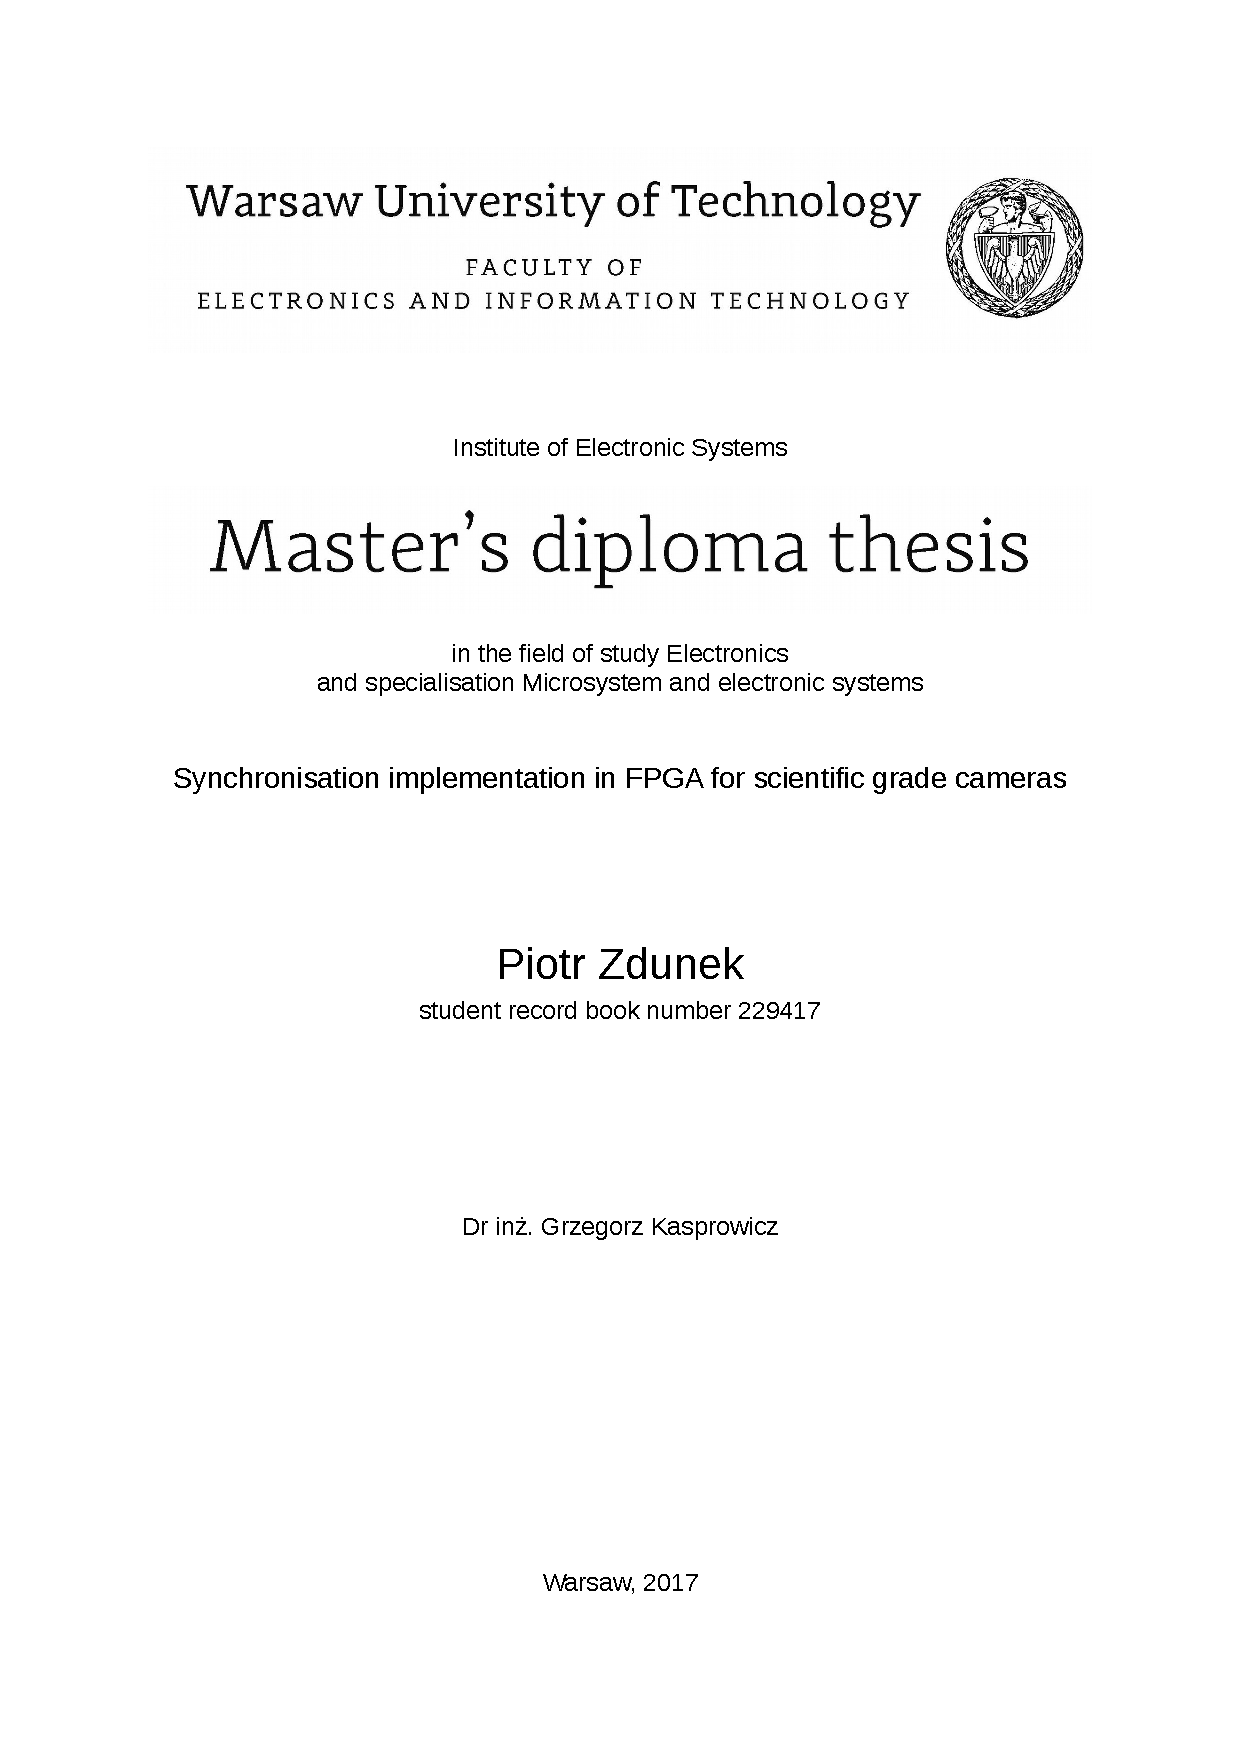
\includepdf[pages=-]{./titlepage/titlepage.pdf}
\pagestyle{empty}
%\setcounter{savepage}{\thepage}
% First copy: start a new page, and save the page number.
\cleardoublepage
% Uncomment the next line if you do NOT want a page number on your
% abstract and acknowledgments pages.
%\pagestyle{empty}
%\setcounter{savepage}{\thepage}
%

%\cleardoublepage
%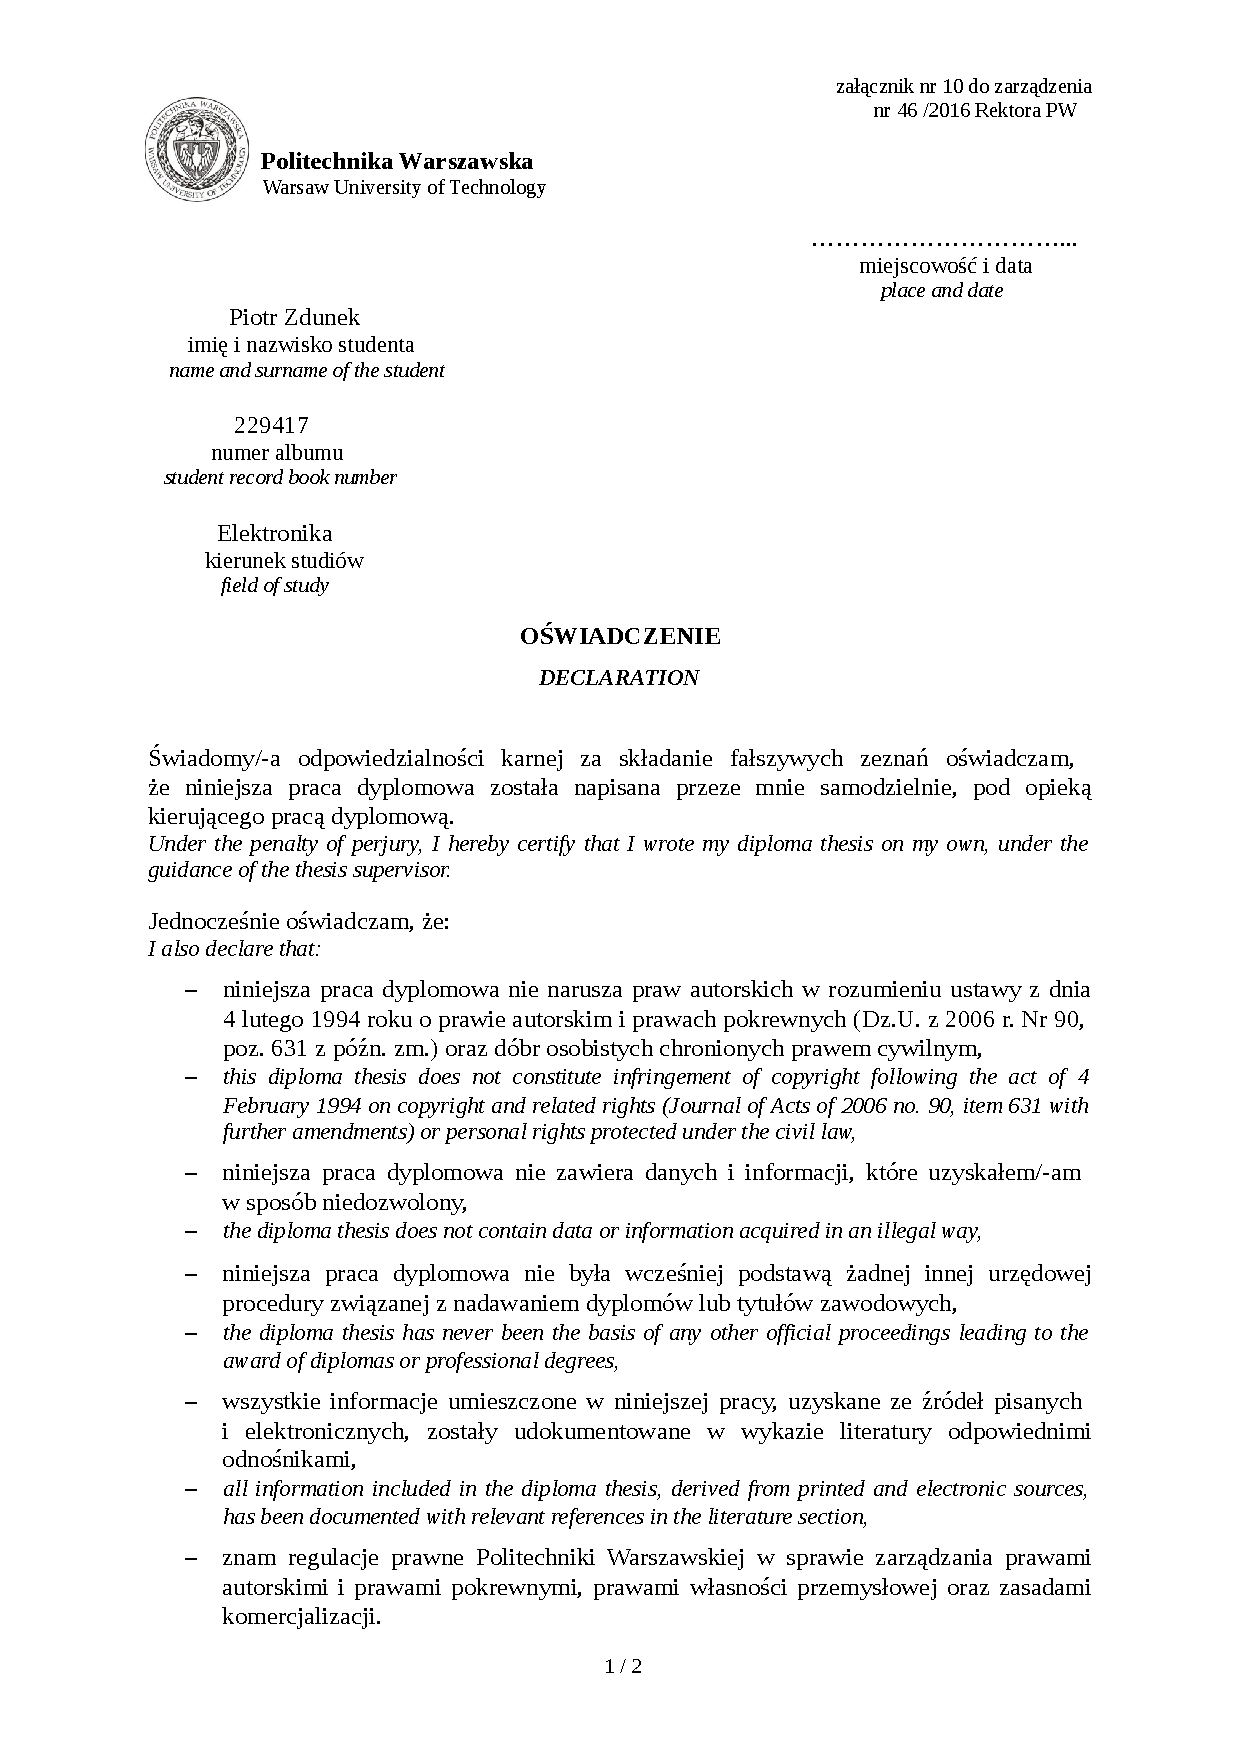
\includepdf[pages=-]{./titlepage/osw.pdf}
%s\pagestyle{empty}
%\setcounter{savepage}{\thepage}
%% First copy: start a new page, and save the page number.
%%
%
%\cleardoublepage\null
%%

%\begin{abstractpage}
%% $Log: abstract.tex,v $
% Revision 1.0  11.2015 % 
% 
%
%% The text of your abstract and nothing else (other than comments) goes here.
%% It will be single-spaced and the rest of the text that is supposed to go on
%% the abstract page will be generated by the abstractpage environment.  This
%% file should be \input (not \include 'd) from cover.tex.

%Original text:
%In this thesis, I designed and implemented a compiler which performs
%optimizations that reduce the number of low-level floating point operations
%necessary for a specific task; this involves the optimization of chains of
%floating point operations as well as the implementation of a ``fixed'' point
%data type that allows some floating point operations to simulated with integer
%arithmetic.  The source language of the compiler is a subset of C, and the
%destination language is assembly language for a micro-floating point CPU.  An
%instruction-level simulator of the CPU was written to allow testing of the
%code.  A series of test pieces of codes was compiled, both with and without
%optimization, to determine how effective these optimizations were.


In this Master Thesis a Scientific Camera framework design is presented. As far as an embedded system design is
concerned, scientific cameras present a great engineering effort in order to succesfully design and implement this kind
of device. This is why this framework was created, so that an engineer wanting to quickly test his or her design can
benefit from it. Proposed framework is build using Xilinx Zynq SoC and thus allows for creating a camera that has 
a multigigabit data acquisition capability as well as multigigabit transmission using SATA or 10 GbE interfaces. 
What is more, a designer can benefit from using a heterogenous operating system where on a multicore processor 
one core is running a real-time operating system whereas on the second core an embedded Linux operating system is 
being run. This provides a great deal of possibilites for numerous applications. Another feature of the framework is 
the multichannel support where multiple cameras can be synchronised using either a dedicated MLVDS interface or 
Ethernet based Precision-Time-Protocol. Mentioned features given as a tested and ready to use subsusystems of a Xilinx 
Vivado project allows for quicker and less error prone scientific camera design. Project is targeted specifically 
towards scientific camera systems due to the fact that this market is very broad and every project has different
requirements. What is common in all scientific camera projects is the sensor data acquisition, synchronisation
capability as well as data transmission. This proves that such a framework can greatly speed up the development 
of a scientific camera. 

%\end{abstractpage}
%

\cleardoublepage
% $Log: abstract.tex,v $
% Revision 1.0  11.2015 % 
% 
%
%% The text of your abstract and nothing else (other than comments) goes here.
%% It will be single-spaced and the rest of the text that is supposed to go on
%% the abstract page will be generated by the abstractpage environment.  This
%% file should be \input (not \include 'd) from cover.tex.

%Original text:
%In this thesis, I designed and implemented a compiler which performs
%optimizations that reduce the number of low-level floating point operations
%necessary for a specific task; this involves the optimization of chains of
%floating point operations as well as the implementation of a ``fixed'' point
%data type that allows some floating point operations to simulated with integer
%arithmetic.  The source language of the compiler is a subset of C, and the
%destination language is assembly language for a micro-floating point CPU.  An
%instruction-level simulator of the CPU was written to allow testing of the
%code.  A series of test pieces of codes was compiled, both with and without
%optimization, to determine how effective these optimizations were.


In this Master Thesis a Scientific Camera framework design is presented. As far as an embedded system design is
concerned, scientific cameras present a great engineering effort in order to succesfully design and implement this kind
of device. This is why this framework was created, so that an engineer wanting to quickly test his or her design can
benefit from it. Proposed framework is build using Xilinx Zynq SoC and thus allows for creating a camera that has 
a multigigabit data acquisition capability as well as multigigabit transmission using SATA or 10 GbE interfaces. 
What is more, a designer can benefit from using a heterogenous operating system where on a multicore processor 
one core is running a real-time operating system whereas on the second core an embedded Linux operating system is 
being run. This provides a great deal of possibilites for numerous applications. Another feature of the framework is 
the multichannel support where multiple cameras can be synchronised using either a dedicated MLVDS interface or 
Ethernet based Precision-Time-Protocol. Mentioned features given as a tested and ready to use subsusystems of a Xilinx 
Vivado project allows for quicker and less error prone scientific camera design. Project is targeted specifically 
towards scientific camera systems due to the fact that this market is very broad and every project has different
requirements. What is common in all scientific camera projects is the sensor data acquisition, synchronisation
capability as well as data transmission. This proves that such a framework can greatly speed up the development 
of a scientific camera. 
 %summary
\cleardoublepage
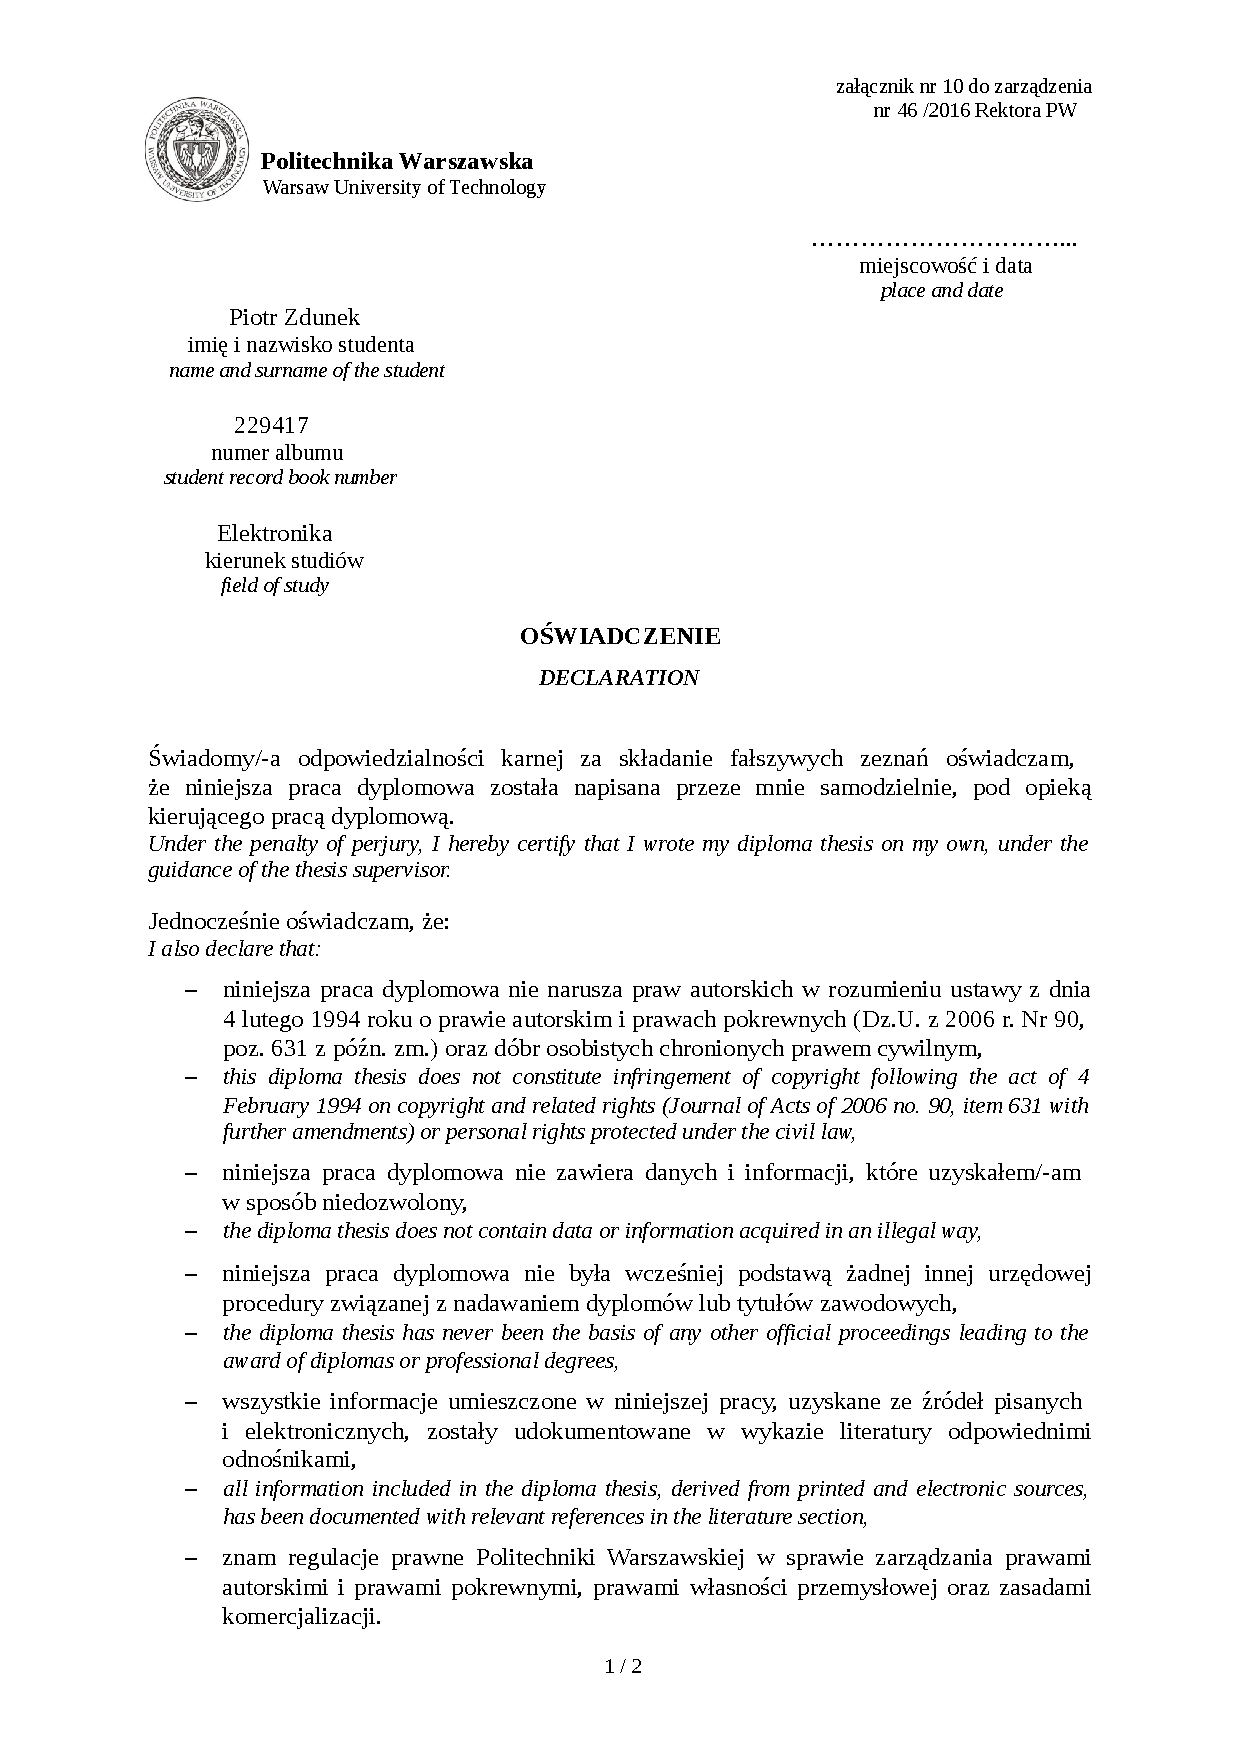
\includepdf[pages=-]{./titlepage/osw.pdf}
\pagestyle{empty}
\cleardoublepage
\tableofcontents
\newpage

%\body

\chapter{Introduction}

\lipsum[3-56]
\section{Project genesis}
\section{Motivation and Objectives}
\subsection{Literature review}
\subsection{Market review} 
\section{Requirements}
%Compact, low weight, high speed, two different sensors, rugged
\section{Thesis statement} 
%Make an embedded camera and evaluate the use of high-speed interfaces for hyper-spectral aerial applications. 

%Here the whole genesis and the requirements of the projects are stated and defined. 
%After reading this chapter, the reader must understand what is going to be designed. 
%\chapter{Genesis}

In this master thesis an implementation of Precision-Time-Protocol Timestamping Unit in FPGA fabric for scientific
camera systems is presented. The project was completed at Photonics and Web Engineering Group at the Institute of 
Electronics Systems which has a significant contribution to X-ray measurement research (TODO publikacje).  Having a scientific cooperation with
another Polish university, there was a need to develop hardware and firmware for novel extremely high-speed,
multichannel, X-ray silicon based camera. This project is undergoing a patent application, and for this reason the 
detailed description of the project cannot be included in this thesis. 

Specifically, a time synchronisation system providing an accurate UTC time was required in order to correctly control
the exposure time between the systems' channels.  This master thesis focuses on that aspect of the project.   


\section{Problem statement}
Providing an accurate timestamping for modern scientific grade camera system is a \textbf{complicated engineering
problem}. The designed hardware for the camera system used Xilinx Zynq SoC\cite{XIL:ZYNQ} which has built
in timestamping capability in the Media Access Controller (MAC). Nevertheless, the timestamping register is not available for
to be read by the operating system and programmable logic \cite[16.4.2]{XIL:ZYNQ_TRM} and the provided functionality of timestamping from
Xilinx is limited and provides low accuracy \cite[16.2.7]{XIL:ZYNQ_TRM} and significant jitter \cite{XIL:PTP_TESTS}. 
Xilinx User Guide Number 585 - Technical Rerence Manual explicitly mentions the fact that the Timestamping Unit can be 
implemented in hardware (programmable logic) in order to achieve better accuracy. This has not been done before and 
this thesis provides the solution to the mentioned problem. 

\section{Solution}
The solution for the problem is to design a Timestamping Unit (TSU) in digital system in FPGA fabric for the Zynq SoC
and use the MAC's built in PTP filtering capability to use this IP Core as a replacement for the internal built in TSU.
What is more, an Ethernet driver modification is required to exchange the TSU and an external oscillator has to be added
to the system in order to precisely run the counters in the TSU. 

\section{Statement of Originality}

This solution provides a way to perform PTP based time synchronisation using Zynq SoC. There are
other methods which provide time synchronisation of different precision such as:
\begin{itemize}
    \item GPS
    \item NTP - precision of up to
    \item PTP (by standard) - sub-milisecond precision 
    \item White Rabbit - sub-nanosecond precision 
\end{itemize}

Nevertheless, the solution provided in this master thesis is \textbf{original}. Standard PTP in the
Zynq SoC does not function properly and in order to be able to use PTP on Zynq with high precision and low jitter,
TSU needs to be implemented in digital fabric.  


\chapter{Concept of design}
In this chapter a concept of the design of the camera is presented. First of all, main camera requirements are shown and juxtaposed with possible solutions. Afterwards the specification of the design is described in detail.

\section{Main requirements}

\begin{itemize}
\item Framerate at 100 fps at 2048 x 2048 resolution
\item High speed interface 
\item Processing capability
\item Possible IMU integration
\end{itemize}

\section{Specification}

\begin{itemize}
\item Framerate at 180 fps at 2048 x 2048 resolution
for CMV4000 and 100 fps for CIS1910F
\item 6.25 Gbps interfaces: SDI, CoaXPress, Aurora, PCie
\item FPGA fabric for processing ability
\item RS485 for communication with IMU and master controller

\end{itemize}

%How are we going to design it and what do we want to test
%\chapter{Requirements}

\begin{itemize}
    \item provide timestamping capability with accuracy in ns range, better than built-in solution provided by Xilinx
    \item timestamping register value should be available by operating system and programmable logic


\end{itemize}

\chapter{Camera development}




%The development of the camera. 
\chapter{Evaluation of high speed interfaces for aerial hyper-spectral camera}


In this chapter an evaluation of high speed interfaces for aerial hyper-spectral application is presented. Firstly, the hypothesis of the evaluation is stated, then two high speed interfaces are used for hypothesis testing. At the end the results of the study are presented. 
%The tests of high speed interfaces.
\chapter{Summary}
In this chapter the summary of the master thesis is presented. Firstly the thesis objectives are contrasted with the final results. Then the main aspects of the work are shown with the description of possible future work. At the end the final summary is shown. 

\section{Thesis objectives and results}
\section{Future work}
\section{Final summary}
%What is the outcome?

\addcontentsline{toc}{chapter}{Bibliography}
\bibliographystyle{alpha}
\bibliography{bibliography/bibliography}

%glossary
%table of pictures 
%list of appendices

\appendix
% appendices come here




\end{document}
